
\section{The Large Hadron Collider}
\label{sec:cmsexperiment:lhc}

% overview
The \acrfull{lhc} \cite{exhep:lhc:Evans:2008zzb} is a 27 km circular particle collider located at the \acrfull{cern} across the border between France and Switzerland. The LHC was constructed during 1998-2008 in a 100-meter-deep underground tunnel previously used by the \acrfull{lep} \cite{exhep:lep:Myers:1991ym}. Inside the LHC, two proton beams collide at a maximum center-of-mass energy of $\sqrt{s}=14$ TeV with a designed instant luminosity of \SI{e34}{\per\cm\squared \per\s}. Around the ring path of the LHC, four collision positions are designed corresponding to four LHC experiments: CMS \cite{exhep:cms:Chatrchyan:2008aa} (Point 5), ATLAS \cite{exhep:atlas:Aad:2008zzm} (Point 1), LHCb \cite{exhep:lhcb:Alves:2008zz} (Point 8) and Alice \cite{exhep:alice:Aamodt:2008zz} (Point 2).


% constituents
The main components of LHC include two tubes with ultrahigh vacuum and about ten thousand superconducting magnets with various sizes installed alone the ring, including 1232 dipole magnets with length of 15 m to bend the beams and 392 quadrupole magnets with length of 5-7 m to focus the beams \cite{exhep:lhcFactsFigures}. Magnets of higher multipole orders are also used for corrections of the magnetic field. A liquid helium cooling system is used to cool the superconducting electromagnets at a cryogenic temperature of -271.3 \si{\degreeCelsius}. 


\begin{figure}[ht]
    \centering
    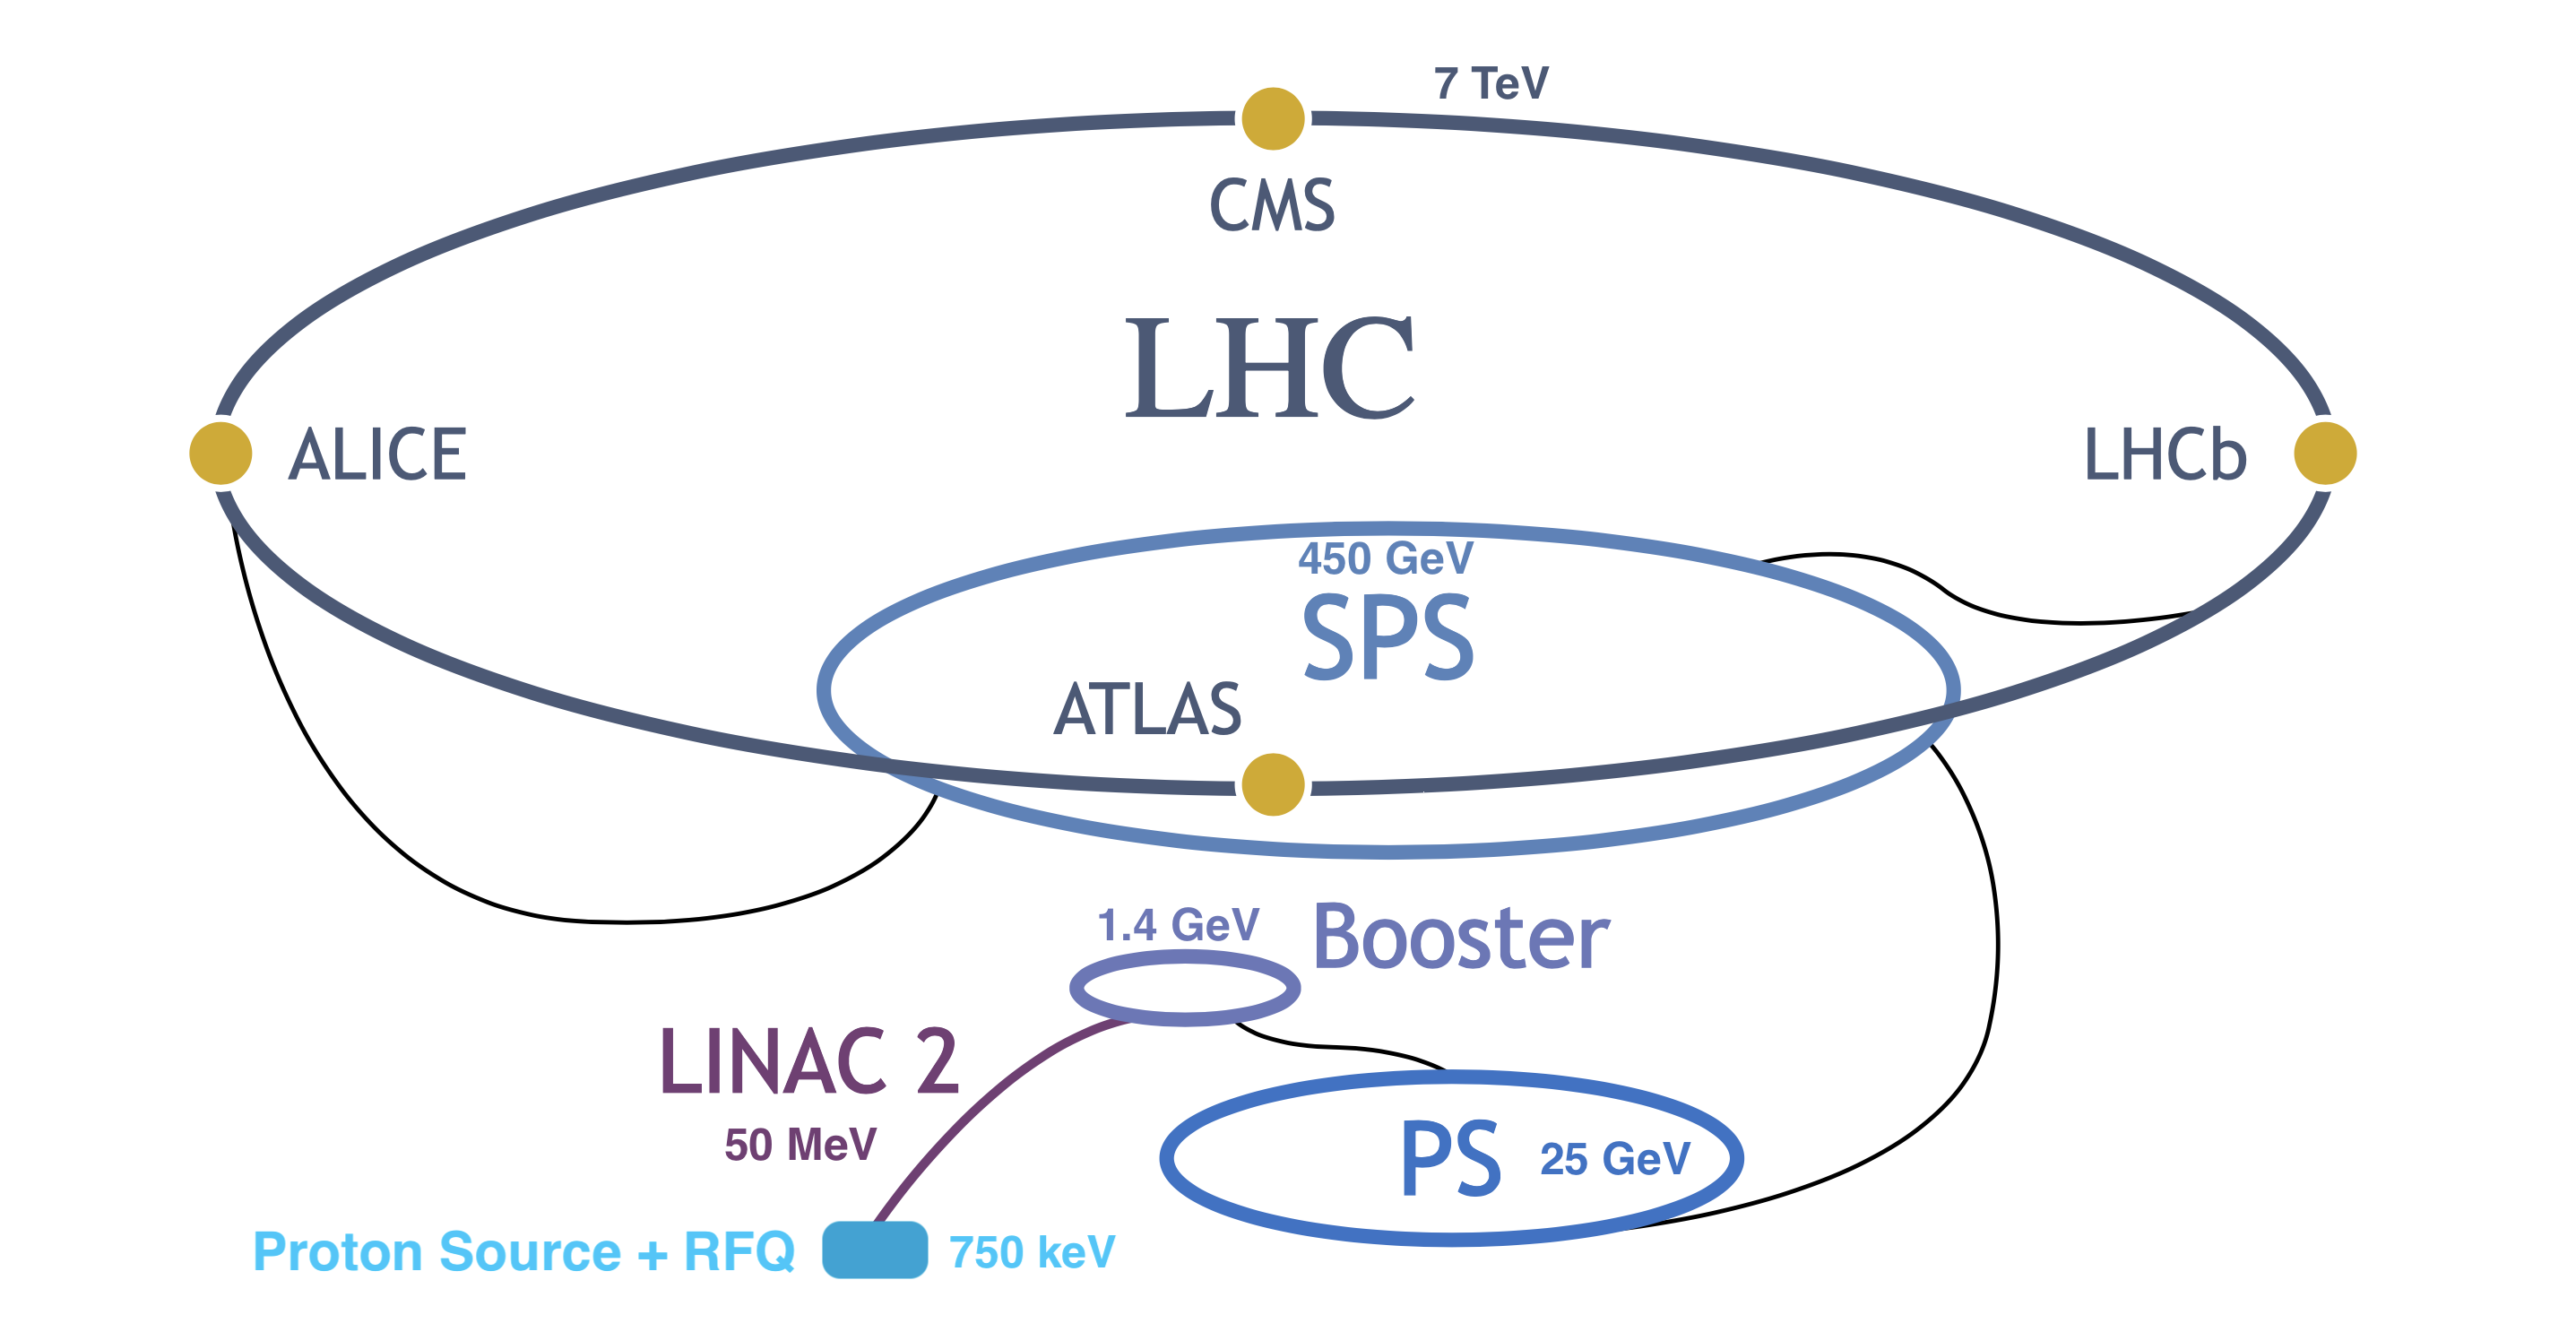
\includegraphics[width=0.8\textwidth]{chapters/CMSExperiment/sectionLHC/figures/lhc.png}
    \caption{Schematic overview of the LHC and related accelerator complex. The accelerator chain includes proton source, \acrfull{rfq}, LINAC, \acrfull{psb}, \acrfull{ps}, \acrfull{sps}, and finally the LHC \cite{exhep:lhcInject:Benedikt:2004wm}. Around the ring path of the LHC locate four LHC experiments: CMS \cite{exhep:cms:Chatrchyan:2008aa} (Point 5), ATLAS \cite{exhep:atlas:Aad:2008zzm} (Point 1), LHCb \cite{exhep:lhcb:Alves:2008zz} (Point 8) and Alice \cite{exhep:alice:Aamodt:2008zz} (Point 2)}
    \label{fig:cmsexperiment:lhc:map}
\end{figure}


% beam pipe
Before injected into the LHC, protons are accelerated to 450 GeV by a few existing accelerator facilities at CERN. Figure~\ref{fig:cmsexperiment:lhc:map} shows a schematic overview of the LHC with its related accelerator complex at CERN \cite{exhep:lhcInject:Benedikt:2004wm}. First, protons are produced by the ionization hydrogen gas and are extracted by a 90 keV voltage to inject into the \acrfull{rfq} where protons are divided into bunch crossings and are accelerated to 750 keV. A linear accelerator (Linac2) then energizes them to 50 MeV. The \acrfull{psb}, which has four superimposed synchrotron rings, brings the protons to 1.4 GeV for the injection to the \acrfull{ps}, a 628 m synchrotron outputting beams with energy of 25 GeV. The \acrfull{sps} further boosted to 450 GeV in its 7-km-long ring and deliver the beam to LHC. When accelerating proton beam from 450 GeV at the LHC injection to 6.5 TeV for the physics collision in the Run-2, the dipole magnetic field is increased from 0.54 T to 7.7 T to increase the banding power to circulating energized beams. During a physics run, luminosity of LHC decays with a lifetime about 14.9 hours \cite{exhep:lhc:Evans:2008zzb} due to effects of physics cross-section, photon emittances alone the circular path and scattering off the air remains. Therefore, every one or two days



% operation schedule
The operation of LHC from 2010 to 2035 consists of 6 runs with shutdown periods for upgrading and maintenance during the run intervals. In the Run-1 from 2010 to 2013, LHC delivered about 6 $fb^{-1}$ pp collision at $\sqrt{s}=7$ TeV in 2010, 2011 and 23.3 $fb^{-1}$ pp collision at $\sqrt{s}=8$ TeV in 2012 \cite{cms:publicLumiInfo}, with which the discovery of Higgs boson was made by the ATLAS \cite{exhep:atlasHiggsDisc:Aad:2012tfa} and the CMS \cite{exhep:cmsHiggsDisc:Chatrchyan:2012ufa}. In the Run-2 from 2016 to 2018, LHC produced 144 $fb^{-1}$ pp collisions at $\sqrt{s}=13$ TeV \cite{cms:publicLumiInfo}. Currently in 2020, the LHC is in its second long shutdown period, expecting Run3 starting in 2021 to operate at the maximum collision energy of $\sqrt{s}=14$ TeV. After Run3, LHC will be upgraded to higher luminosity or the \acrfull{hllhc} to reach an instant luminosity of \SI{5e34}{\per\cm\squared \per\s}, five times as much as current value. In the era of HL-LHC, three extra runs are scheduled during 2026-2035. In the long term future beyond the HL-LHC era, the \acrfull{fcc} \cite{exhep:fcc:Benedikt:2715354} plan is proposed to build a 100 km hadron collider next to the LHC and further increase the collision energy to the level of 100 TeV.